\subsection{System Structure And Parametrisation}\label{sec:SSP}

The central goal of the INTO-CPS Application is to enable the composition and co-simulation of a system consisting of one or more FMUs. 
The use of the FMI standard enables exchange at the level of the individual FMUs.
However, it does not describe an exchange format for composing and parametrising a simulation scenario consisting of multiple FMUs.
Due to the lack of an established standard, the INTO-CPS Application uses its own ad-hoc format referred to as the \emph{multi-model} format.

Recently a new companion standard to FMI was published: the \emph{System Structure and Parameterization} (SSP) standard~\cite{SSP19}\footnote{\url{https://ssp-standard.org/}}.
The standard uses a zip-based packaging format similar to FMI, where multiple artefacts are bundled into a single package referred to as a \emph{SSP package} -- each representing a ready to simulate system.
An obvious benefit of adopting this standard is exchangeability of complete systems between tools. Currently only a few such as OpenModelica and \emph{FMPy}\footnote{\url{https://github.com/CATIA-Systems/FMPy}}, however given its close relation to FMI, it seems likely that more tools will adopt it. 
An example of what the running example may look like when bundled as a package is seen on Figure~\ref{fig:ssp_structure}.

The standard covers the functionality present in the existing format, but also adds several capabilities which are useful for the INTO-CPS Application.
Additionally, there are also some important semantic differences between the existing format and SSP.
Ultimately, some of these influence the interaction in the GUI editor, as such the most relevant differences are highlighted below.

\begin{description}
\item[Components and Hierarchy:]
While the standard is closely aligned with the FMI it is not limited to describing systems purely consisting of FMUs.
Instead the standard establishes the concept of a \emph{component} -- an atomic block of the system, which is backed by some underlying implementation.
For example, a component may reference a FMU as its implementation.
A component may itself be a SSP package, which in this context, is referred to as a \emph{sub-system}. 
The latter enables the creation of hierarchies of components.


\item[Parameterization:]
There is an important difference between how parameters are treated in a multi-model and by SSP.
In the former all parameters are defined inline, there is no mechanism to reference a ``shared'' parameter from multiple components.
SSP on the other hand provides the \emph{parameter sets} and \emph{parameter mappings} concepts which makes it possible to declare a set of parameters and then bind these to the concrete components\footnote{Inside the SSP standard these are referred to as System Structure Parameter Values and System Structure Parameter Mappings.}.

\item[Extensibility:]
Similar to FMI the standard is largely based on XML and is designed to be extensible through three types of extension mechanisms: Annotations, extra files and MIME type-based format dispatch.
This allows for the creation of new extensions to the standard referred to as \emph{layered standards}.
A potential use case of this is to extend the standard with support for semantic adaptations.
\end{description}

%Annotations can be applied to several XML elements, for example a component. The annotation may contain arbitrary XML data.


%\begin{figure}[bt]
%\centering
%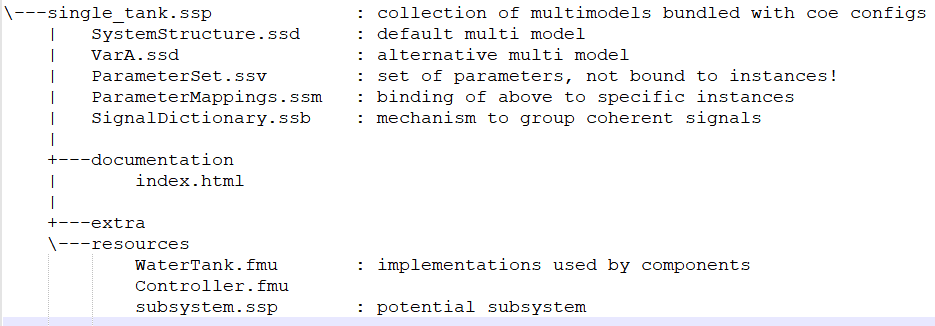
\includegraphics[width=\columnwidth]{Images/ssp_structure.png}
%\caption{}
%\label{fig:ssp_structure}
%\end{figure}



\begin{figure}[bt]
\centering

\begin{Verbatim}[tabsize=4,fontsize=\small,samepage=true,frame=single]
\---single_tank.ssp         : collection of multi models
    | SystemStructure.ssd   : default multi model
    | VarA.ssd              : alternative multi model
    | ParameterSet.ssv      : set of parameters
    | ParameterMappings.ssm : binding params to instances
    | SignalDictionary.ssb  : mechanism to group signals
    |
    +---documentation
    | index.html
    |
    +---extra               : extra files extension mechanism
    |
    \---resources           : implementations of components
      WaterTank.fmu
      Controller.fmu	
      subsystem.ssp         : potential subsystem
\end{Verbatim}

\caption{Example of the file structure of the running example stored as a SSP package. 
The comments on the side describe the role of the file. }
\label{fig:ssp_structure}
\end{figure}
%\begin{figure}[bt]
\centering
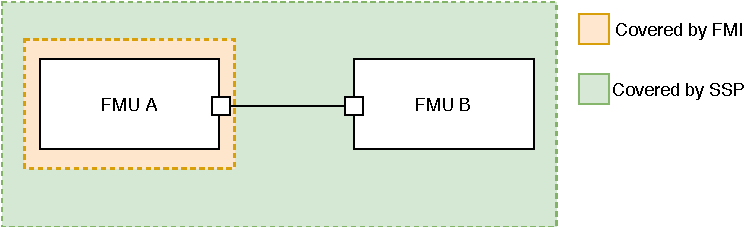
\includegraphics[width=0.8\columnwidth]{Images/fmi_vs_ssp.pdf}
\caption{Graphical depiction of domains that the FMI and SSP standards covers.
FMI describes the interface of the individual blocks. SSP defines the instances and connectivity of the FMUs}
\label{fig:fmi_vs_ssp}
\end{figure}

%A more in-depth discussion of the difference and migrations between the current and new format can be found in section~\ref{ssec:mm_vs_ssp}.


%However, when the application was initially developed no standard existed which describe how the individual FMUs %may be composed and parametrized.
%A graphical depiction of the domains covered by FMI and SSP can be seen in figure~\ref{fig:fmi_vs_ssp}.
%Adopting the new standard has clear benefits such as improving exchangeability between tools, being more %expressive and extensible than the current format.

%It is the a clear ambition of the developers of the INTO-CPS tool-chain to adopt SSP as the preferred format for %describing co-simulation scenarios.
%As such the rest of the paper assumes that the capabilities present in SSP is available for the graphical editor.